\documentclass[11pt,twocolumn]{article}

\usepackage[margin=1in]{geometry}
\usepackage{graphicx}
\usepackage{amsmath,amssymb}
\usepackage{hyperref}
\usepackage{array}
\usepackage{natbib}
\usepackage[backend=biber]{biblatex}
\addbibresource{sources.bib}

\newcommand{\coursefootnote}{
  \renewcommand{\thefootnote}{\fnsymbol{footnote}}
  \footnotetext[1]{Course Project for DS-6051 -- Decoding Large Language Models.}
  \renewcommand{\thefootnote}{\arabic{footnote}}
}

\title{
  \textbf{Brains in Bits: A Comparative Study of PEFT Techniques for Commonsense Reasoning on GPT-2}
  
}
\author{
Vishwanath Guruvayur \\
University of Virginia \\
\texttt{vish@virginia.edu}
\and
Luke Napolitano \\
University of Virginia \\
\texttt{ljn5yms@virginia.edu}
\and
Doruk Ozar \\
University of Virginia \\
\texttt{bcp8dm@virginia.edu}
}

\date{}

\begin{document}

\maketitle
\coursefootnote   % This inserts the footnote exactly once

\begin{abstract}
While industry convention has assumed that the bigger, the better, training large models fully is resource-intensive, often impractical, and costly to the environment according to recent research \cite{Patterson2022}. In this project, we investigate how smaller models like GPT-2 can be selectively enhanced for common-sense reasoning tasks through Parameter-Efficient Fine-Tuning (PEFT) methods, reducing the cost and enhancing the impact of LLM research and use.

We compared four PEFT techniques: LoRA, QLoRA, Prefix Tuning and IA³. Instead of updating all model parameters, these methods selectively adjust small, critical parts of the model, particularly within its attention mechanisms. Our results show that IA³ and Prefix Tuning substantially outperform LoRA and QLoRA, achieving up to 50\% validation accuracy in commonsense categories, with noticeable reductions in perplexity. Each of the four methods, applied to the smallest available GPT-2 model, outperform the largest GPT-2 model in a zero-shot test of common-sense reasoning.

These findings suggest that PEFT methods can meaningfully strengthen specific reasoning capabilities even in smaller, open-source versions of the multi-billion parameter proprietary LLMs. Our work supports the idea that modular, targeted training strategies could form a scalable alternative to LLM training that significantly reduces the environmental and computational impact that off-the-shelf multi-billion parameter models currently offer. Future directions include expanding to ensemble PEFT methods and scaling experiments to other models such as Quen 3, Llama 4, and Mistral 3.1.
\end{abstract}

\section{Introduction}
\label{sec:intro}

\indent The release of ChatGPT in late 2022 brought about a wave of LLM advancements that have seemed to follow a trend: bigger is better. Recently, a new proprietary model is released almost every month with more parameters and purportedly better performance than any model before it. However, as these top-of-the-line models have gotten more advanced, they have continued to become more expensive to train and use. 

Current approaches often involve training ever-larger models using massive datasets and computational resources. However, this brute-force strategy raises practical concerns about scalability, accessibility, and interpretability. Fine-tuning such large models from scratch is increasingly impractical, especially for smaller research groups or applications that need specialized adaptation.

In this project, we investigate whether the performance of more accessible models like a small GPT-2 notably improves by using Parameter-Efficient Fine Tuning (PEFT) techniques when applied to a very specific task like MCQ answering. Rather than updating millions of parameters, PEFT methods selectively adapt a small subset of components, particularly within the model's attention mechanisms, which can be thought of as the `brain' of LLMs.

Our primary objectives are threefold:
\begin{itemize}
    \item Assess whether PEFT methods can inject common sense reasoning capabilities into a basic LLM.
    \item Compare the effectiveness of different PEFT strategies (LoRA, Prefix Tuning, IA³, and QLoRA) in improving model performance.
    \item Understand how different types of reparametrization and adaptive techniques affect different cognitive abilities of the LLM Transformer Architecture.
    \item Reflect on the broader implications of modular training approaches for LLM research and general use.
\end{itemize}

By studying how small, controlled updates can meaningfully improve commonsense reasoning, we hope to gain insights into how structured cognitive skills might be cultivated in language models without the need for massive retraining or scaling alone.



\section{Related works}
\label{sec:background}

The development of efficient fine-tuning strategies for Large Language Models (LLMs) has been an active area of research, particularly as model sizes and training costs continue to grow.

\textbf{A Critical Review of PEFT} \cite{Xu2023} covered the history of parameter-efficient fine-tuning techniques, their applications, and future direction for LLM training and tuning. The use of PEFT seems to improve parameter efficiency and reduce computational requirements.

\textbf{LoRA and QLoRA} \cite{Noble2023} explained how LoRA freezes the original weights of the model and adds a low-rank matrix that is tuned to the context. The author also briefly covered how QLoRA quantizes low-rank matrices to a lower precision.  

\textbf{Prefix Tuning} \cite{Razavi2023} summarized the addition of a learned prefix tokens to the beginning of a model's processing pipeline that help guide the model's behavior.

\textbf{IA³ (Input-Adaptive Attention)} \cite{Liu2022} extended these ideas by learning input-dependent scaling factors inside the attention and feedforward modules. IA³ showed particular promise for few-shot fine-tuning, achieving competitive results with significantly fewer trainable parameters.

Most prior work evaluated PEFT techniques on instruction-following, summarization, or dialogue tasks. However, their application to \textit{commonsense reasoning} which is a core component of AGI remains rather underexplored. Our project contributes by systematically comparing these PEFT methods on the CommonsenseQA benchmark, focusing on the ability to teach implicit world knowledge to a relatively small model like GPT-2.



\section{Methodology}
\label{sec:methodology}
In this section we will discuss our approach to experiment with different PEFT methods for our finalized Dataset.

\subsection{Data: CommonsenseQA}
Our initial experiments aimed to fine-tune GPT-2 on the OpenMathInstruct-2 dataset for mathematical reasoning. However, due to GPT-2's limited capacity to understand complex symbolic structures, training stalled at a high loss value of 6.6 without notable accuracy improvements.

We did not want to move to a larger model like Mistral 6B Instruct Model because we wanted to test the capabilities of PEFT methods in a very basic GPT like GPT-2 and not have any beneficiary aspects of having a larger model.

Recognizing the mismatch between task complexity and model capacity, we pivoted to \textbf{CommonsenseQA}, a multiple-choice question-answering dataset focused on everyday commonsense knowledge. Each sample in CommonsenseQA consists of a question and five candidate answers, with exactly one correct choice. The dataset is designed to challenge models on reasoning about implicit world knowledge rather than relying purely on surface-level patterns, making it a suitable benchmark for our objectives.

The dataset also has 785 categories of these common sense questions. We clustered these categories into a larger set of 10 broad classes to better understand the proficiency each method shows in these broader common sense classes.

\subsection{Model: GPT-2 with PEFTs}
We selected the \textbf{GPT-2 small} model (approximately 125M parameters) as our base architecture. GPT-2's autoregressive nature makes it naturally effective at next-word prediction, which aligns well with the multiple-choice format where short, precise outputs are expected. Additionally, GPT-2's manageable size allowed us to conduct multiple fine-tuning experiments within reasonable compute constraints.

\subsection{Parameter Efficient Fine-Tuning Techniques}
We applied and compared four different PEFT methods:
\begin{itemize}
    \item \textbf{LoRA}: Introduces low-rank updates within attention weights.
    \item \textbf{QLoRA}: Combines 4-bit model quantization with LoRA to enable memory-efficient fine-tuning.
    \item \textbf{Prefix Tuning}: Appends learned prefix tokens to each transformer layer’s input.
    \item \textbf{IA³}: Adds learnable scaling factors to the key, value, and feedforward transformations.
\end{itemize}
Each method adapts only a small fraction of the total model parameters, keeping the core model weights frozen.

\begin{figure}[h]
\centering
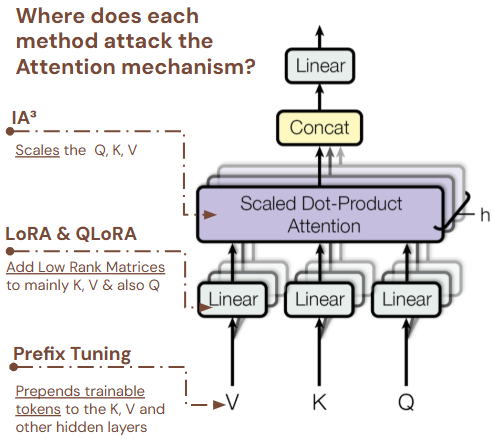
\includegraphics[width=0.5\textwidth]{../graphs/PEFTs.png}
\caption{Intuitive Visualization of the different target regions for each PEFT Method}
\label{fig:peft-target}
\end{figure}

\subsection{Experimental Setup}
We trained all models using a single NVIDIA A100 GPU, leveraging the HuggingFace PEFT library for efficient implementations. Hyperparameters were held consistent across experiments for fair comparison:
\begin{itemize}
    \setlength\itemsep{0em}
    \setlength\parskip{0em}
    \setlength\parsep{0em}
    
    \item Optimizer: AdamW
    \item Learning Rate: 5e-5
    \item Batch Size: 8
    \item Evaluation Strategy: Every 100 steps
    \item Number of Epochs: 10
\end{itemize}

Evaluation was conducted using two primary metrics:
\begin{itemize}
    \item \textbf{Validation Accuracy}: Percentage of correct answers selected. We also calculated this accuracy within the broad classes of questions to understand each method's expertise in specific types of common sense.
    \item \textbf{Perplexity}: A measure of model confidence on validation sequences.
\end{itemize}

To simulate realistic low-resource settings, we limited training to small-to-moderate compute budgets, avoiding large-scale hyperparameter searches.


\section{Experiments and Results}
\label{sec:experiments}

\subsection{Initial Exploration: OpenMathInstruct-2}
Our early experiments on the OpenMathInstruct-2 dataset exposed a fundamental mismatch between GPT-2’s architecture and the demands of mathematical reasoning. Despite extensive training, the model's loss plateaued at approximately 6.6, with minimal improvements in prediction accuracy. This stagnation suggested that the symbolic complexity and structured reasoning required by math datasets exceeded GPT-2’s representational capacity.

\subsection{Strategic Pivot: CommonsenseQA}
Recognizing these limitations, we transitioned to the CommonsenseQA dataset, which emphasizes sentence-level, everyday reasoning—better suited to GPT-2's strengths. This shift allowed us to more accurately assess the effectiveness of parameter-efficient fine-tuning (PEFT) methods without architectural bottlenecks dominating outcomes.

\subsection{Zero-Shot Baseline Performance}
Without fine-tuning, the 1.5B parameter GPT-2 had zero-shot accuracy of roughly 6.35\%—consistent with a five-choice multiple-selection task. This established a clear motivation for targeted fine-tuning on a smaller model.

\subsection{Parameter-Efficient Fine-Tuning (PEFT) Results}
We explored four PEFT methods: \textbf{LoRA}, \textbf{QLoRA}, \textbf{Prefix Tuning}, and \textbf{IA³}. Each method's performance is discussed below, including validation accuracy, perplexity, and training dynamics.

\subsubsection{LoRA}
\textbf{Results}:
\begin{itemize}
    \item Validation Accuracy: \textbf{12\%}
    \item Perplexity: \textbf{14.31}
\end{itemize}

Despite reducing perplexity substantially compared to the zero-shot baseline, LoRA yielded only modest accuracy gains, suggesting limited improvement in reasoning capabilities.
\begin{figure}[h]
\centering
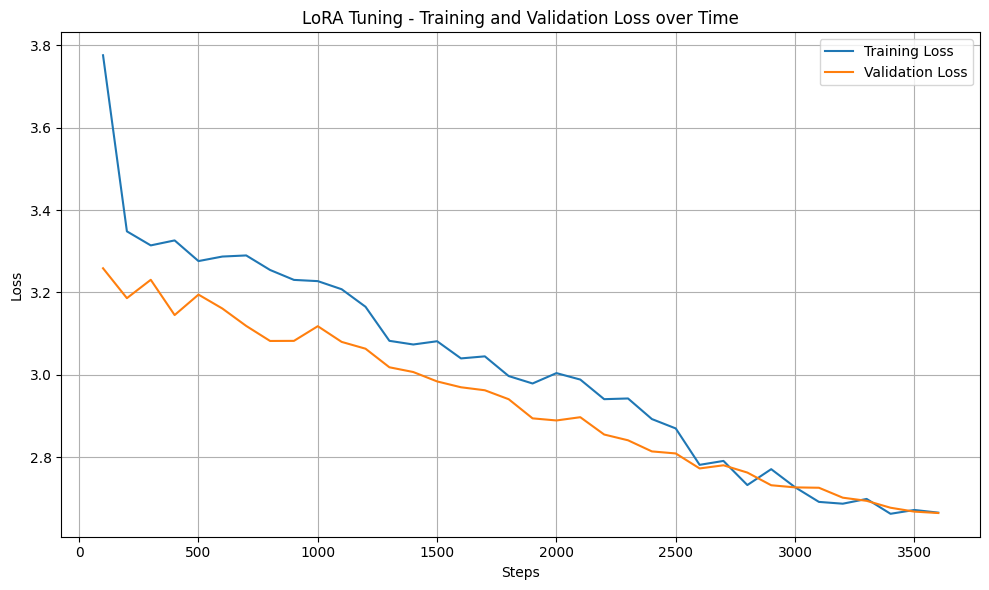
\includegraphics[width=0.45\textwidth]{../graphs/LoRA.png}
\caption{Training and validation loss curves for LoRA fine-tuning.}
\label{fig:lora-loss}
\end{figure}

\subsubsection{QLoRA}
\textbf{Results}:
\begin{itemize}
    \item Validation Accuracy: \textbf{15\%}
    \item Perplexity: \textbf{14.45}
\end{itemize}

QLoRA achieved slightly better accuracy than LoRA with comparable perplexity. However, the improvement remained marginal, reinforcing challenges in adapting GPT-2 to structured reasoning even with quantized fine-tuning.
\begin{figure}[h]
\centering
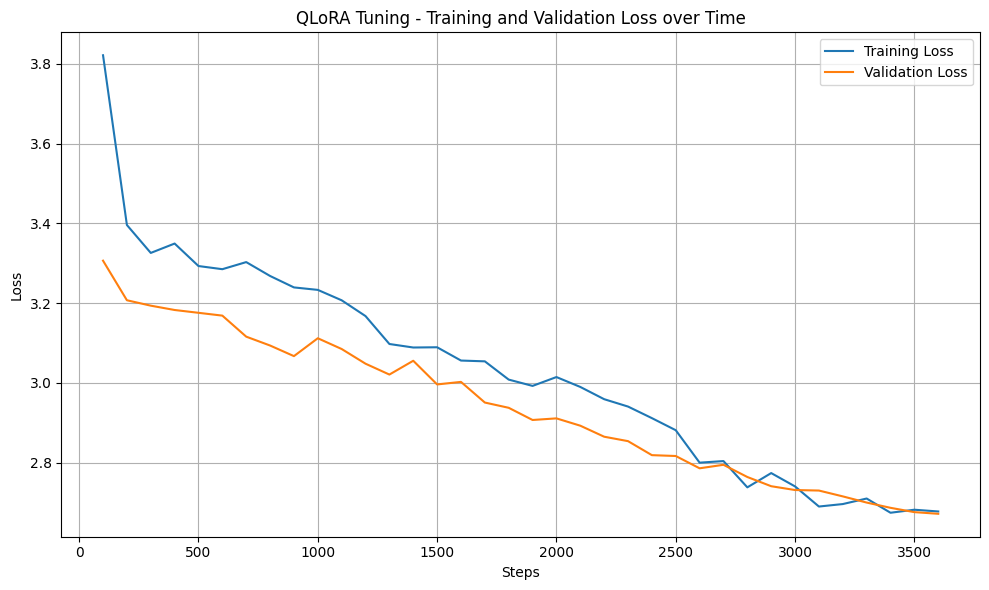
\includegraphics[width=0.45\textwidth]{../graphs/QLoRA.png}
\caption{Training and validation loss curves for QLoRA fine-tuning.}
\label{fig:qlora-loss}
\end{figure}

\subsubsection{Prefix Tuning}
\textbf{Results}:
\begin{itemize}
    \item Validation Accuracy: \textbf{46\%}
    \item Perplexity: \textbf{14.06}
\end{itemize}

Prefix Tuning delivered a major jump in accuracy. Despite only a minor further drop in perplexity compared to LoRA and QLoRA, it enabled much stronger multiple-choice reasoning.
\begin{figure}[h]
\centering
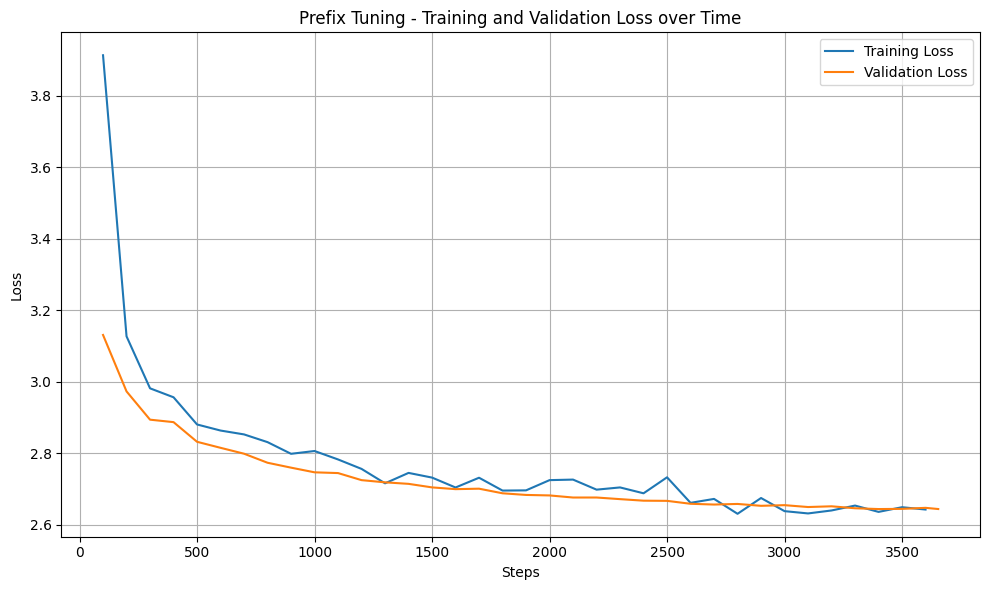
\includegraphics[width=0.45\textwidth]{../graphs/Prefix.png}
\caption{Training and validation loss curves for Prefix Tuning fine-tuning.}
\label{fig:prefix-loss}
\end{figure}

\subsubsection{IA³}
\textbf{Results}:
\begin{itemize}
    \item Validation Accuracy: \textbf{50\%}
    \item Perplexity: \textbf{16.24}
\end{itemize}

IA³ achieved the highest accuracy despite a slightly higher perplexity. This suggests that in CommonsenseQA, perplexity reductions do not fully capture improvements in discriminative reasoning.
\begin{figure}[h]
\centering
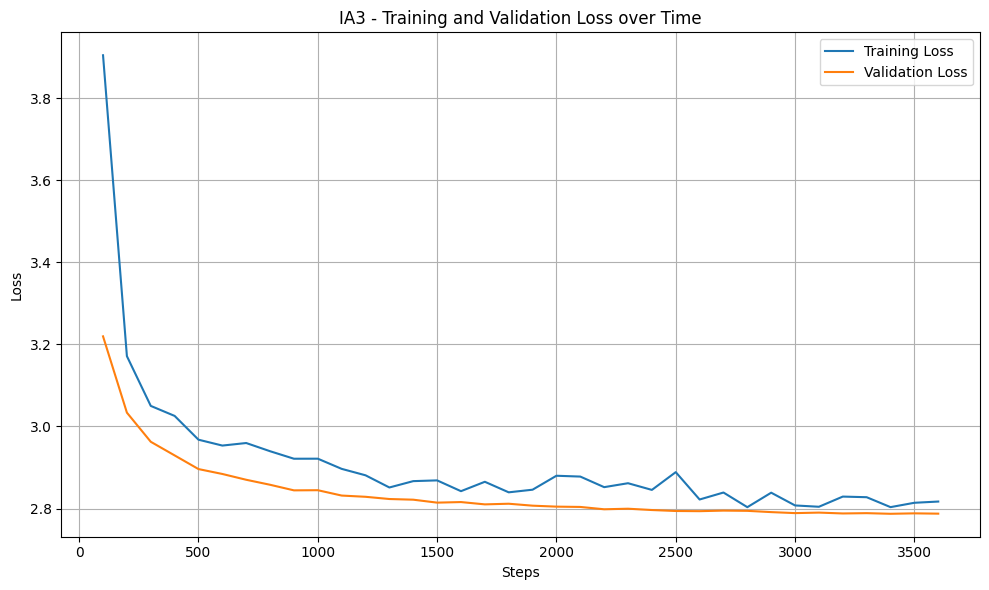
\includegraphics[width=0.45\textwidth]{../graphs/IA3.png}
\caption{Training and validation loss curves for IA³ fine-tuning.}
\label{fig:IA³-loss}
\end{figure}

\subsection{Summary of Metrics}
This is a summary of our experiment results

\newcolumntype{P}[1]{>{\centering\arraybackslash}p{#1}} % centered p-column

\begin{table}[h]
\centering
\renewcommand{\arraystretch}{1.2}
\begin{tabular}{|P{3.3cm}|P{2.7cm}|P{2.3cm}|}
\hline
\textbf{Method} & \textbf{Validation Accuracy (\%)} & \textbf{Perplexity} \\
\hline
Zero-Shot (1.5B) & 6.35\% & 5536.87 \\
LoRA & 12\% & 14.31 \\
QLoRA & 15\% & 14.45 \\
Prefix Tuning & 46\% & 14.06 \\
IA³ & 50\% & 16.24 \\
\hline
\end{tabular}
\caption{Summary of validation accuracy and perplexity across PEFT methods on CommonsenseQA on GPT-2 Small.}
\label{table:summary-metrics}
\end{table}

\subsection{Category-Wise Analysis}

To further probe model behavior, we evaluated category-specific performance across commonsense reasoning types within CommonsenseQA.

\begin{figure}[h]
\centering
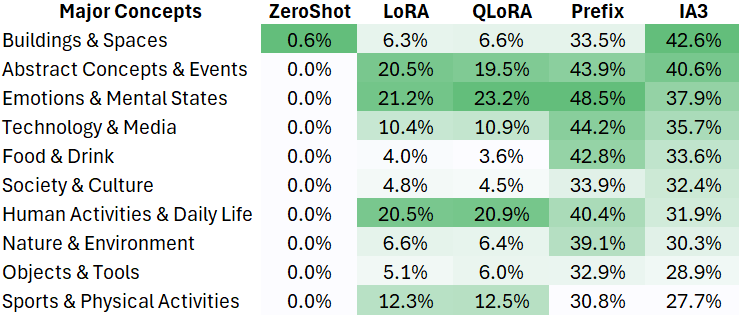
\includegraphics[width=0.5\textwidth]{../graphs/Categorical_Performance.png}
\caption{Validation accuracy by commonsense category across PEFT methods on GPT-2 Small.}
\label{fig:category-accuracy}
\end{figure}

The results suggest that different PEFT methods specialize in different types of conceptual learning.
Prefix Tuning and IA³ show strong capabilities in transferring knowledge to high-level semantic domains like Emotions \& Mental States, Technology \& Media, and Buildings \& Spaces, indicating that they are more effective for complex, abstract reasoning tasks.
In contrast, LoRA and QLoRA offer more modest improvements, suggesting that while they introduce efficiency, they may underfit higher-complexity concepts compared to prefix-based or IA³-based adaptation.

The almost nonexistent performance in the Zero-Shot setting underscores that parameter-efficient fine-tuning is essential when models must generalize to nuanced or structured domains.
Moreover, IA³’s dominance in categories like Buildings \& Spaces hints that task types grounded in physical or spatial reasoning particularly benefit from deeper internal adaptation mechanisms rather than surface-level prompt manipulation.


\subsection{Qualitative Assessment}

Qualitatively, IA³- and Prefix-fine-tuned models showed a stronger grasp of implicit relationships between concepts, often selecting plausible answers even when questions were phrased ambiguously. In contrast, LoRA- and QLoRA-fine-tuned models behaved closer to random guessing, suggesting weaker internalization of commonsense structures.

\subsection{Summary of Findings}

Overall, our experiments demonstrate that \textbf{IA³ and Prefix Tuning are highly effective} for enhancing commonsense reasoning in GPT-2 under resource constraints. While \textbf{LoRA and QLoRA} remain efficient in other contexts, they struggled to deliver meaningful improvements on CommonsenseQA. Of note, however, is that the zero-shot performance of the 1.5B parameter GPT-2 underperformed even PEFT techniques with little impact on common-sense reasoning like LoRA and QLoRA. Smaller open-source models, combined with a weave of robust PEFT techniques thus merit investigation and comparison against other leading models to test how much improvement can be squeezed out of a smaller model.

\section{Discussion}
\label{sec:discussion}
Our results show that Parameter-Efficient Fine-Tuning (PEFT) methods can significantly improve the commonsense reasoning capabilities of smaller language models like GPT-2, but their effectiveness varies significantly across techniques.

\subsection{Interpretation of Results}
IA³ and Prefix Tuning were substantially more effective than LoRA and QLoRA. We hypothesize that this is because IA³ and Prefix Tuning directly intervene in the model’s attention mechanisms, which are central to relational and inferential reasoning. By contrast, LoRA and QLoRA mainly inject low-rank updates into the projection layers, which may be less effective at reshaping internal reasoning processes necessary for commonsense tasks.

The significant drop in perplexity scores for IA³ and Prefix Tuning suggests that these methods help the model gain more confident and structured internal representations of everyday knowledge, even without updating most parameters.

\subsection{Limitations}
While encouraging, our experiments have important limitations:
\begin{itemize}
    \item \textbf{Model Capacity}: GPT-2 small (125M parameters) remains fundamentally limited in its ability to perform deep or multi-hop reasoning.
    \item \textbf{Dataset Simplicity}: CommonsenseQA focuses on relatively shallow commonsense tasks. More nuanced benchmarks could reveal different strengths or weaknesses.
    \item \textbf{Resource Constraints}: All training was conducted under constrained compute budgets, limiting our ability to fully optimize hyperparameters or explore longer training schedules.
\end{itemize}

\subsection{Interesting Observations}
A notable qualitative finding was that Prefix Tuning and IA³ models often selected semantically plausible answers even when wrong, suggesting partial internalization of reasoning heuristics rather than pure memorization. Meanwhile, LoRA and QLoRA-fine-tuned models frequently defaulted to random choices, implying weaker structural learning.

These insights reinforce the view that small, targeted interventions inside the model's cognitive core whic is its attention mechanism, can unlock better reasoning behaviors without requiring full retraining.

\section{Conclusion and Future Work}
\label{sec:conclusion}

This project showed that Parameter-Efficient Fine-Tuning (PEFT) methods can significantly enhance GPT-2's performance on commonsense reasoning tasks without requiring full model retraining. Fine-tuning led to a noticeable increase in accuracy (up to 38\%) and a significant reduction in perplexity score from over 3000 to around 14. Among the techniques explored, IA³ and Prefix Tuning demonstrated substantially better results compared to LoRA and Q-LoRA.

In the future, there are several exciting directions that can be explored. Further exploration of more advanced PEFT techniques, investigation of ensemble strategies that combine different tuning methods, and scaling experiments to larger and more capable language models, such as Mistral, are planned. Additionally, applying these approaches to more challenging and complex datasets could provide deeper insights into their generalization capabilities.


\printbibliography[
heading=bibintoc,
title={References}
]

\end{document}
